\documentclass[border=0pt]{standalone}

\usepackage{enumitem}

\usepackage[sc]{mathpazo}
\usepackage{tikz}
\linespread{1.05}

\newcommand\bluebullet{%
  \tikz[baseline=0ex]\fill[blue!75!black]
    (0,0)--(0.18,0.09)--(0,0.18)--cycle;}


\usepackage[table]{xcolor}
\definecolor{petrol}{RGB}{20,199,211}


\usepackage{tikz}
\usetikzlibrary{calc}


\usepackage{ragged2e}

\begin{document}
\small

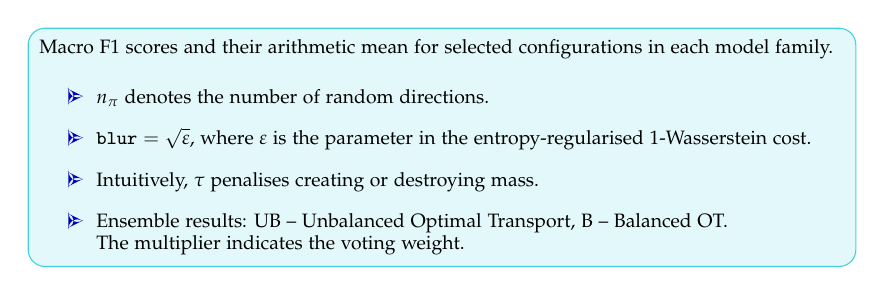
\begin{tikzpicture}
\node[
  draw=petrol!80,              
  fill=petrol!12,              
  rounded corners=6pt,
  minimum width=0.1\linewidth, 
  inner sep=4pt,               
  text width=0.89\linewidth-16pt, 
  font=\scriptsize,
  align=justify                
] (cap) {%
  \noindent Macro F1 scores and their arithmetic mean for selected configurations in each model family.
  
\begin{itemize}[label=\bluebullet,left=1.5em,itemsep=3pt]
\item $n_{\pi}$ denotes the number of random directions.
\item \texttt{blur} \(=\sqrt{\varepsilon}\), where \(\varepsilon\) is the parameter in the entropy-regularised 1-Wasserstein cost.
\item Intuitively, \(\tau\) penalises creating or destroying mass.
\item Ensemble results: UB -- Unbalanced Optimal Transport, B -- Balanced OT.\\The multiplier indicates the voting weight.
\end{itemize}
  };
\end{tikzpicture}

\end{document}